\chapter{Projeto de estudo de Caso}
\label{estudo de caso}

Neste capítulo é apresentado o projeto do estudo de caso. Isso  consiste na elaboração de um protocolo para o estudo de caso, na identificação do problema e na definição das questões e objetivos de pesquisa. O método para coleta dos dados e como eles serão analisados também serão apresentados neste capítulo.

\section{Definição}

Segundo \citeonline{yin2001estudo} o estudo de caso é um conjunto de procedimentos pré-especificados para se realizar um estudo empírico que investiga um fenômeno contemporâneo dentro de seu contexto da vida real, especialmente quando os limites entre o fenômeno e o contexto não estão claramente definidos. Uma grande vantagem do estudo de caso é a sua capacidade de lidar com uma ampla variedade de evidências, documentos, artefatos, entrevistas e observações. Além disso, em algumas situações, como na observação participante, pode ocorrer manipulação informal.

Buscando maior entendimento a respeito do estudo de caso proposto, foram criadas algumas perguntas que são fundamentais para o seu entendimento:

\begin{easylist}[itemize]	
	
	& Qual o escopo do estudo de caso?
	& Qual o problema a ser tratado?
	& Qual a questão de pesquisa relacionada a esse problema?
	& Quais são os objetivos a serem alcançados nessa pesquisa?	
	& Como foi a seleção do estudo de caso?
	& Qual é fonte dos dados coletados nessa pesquisa e qual o método de coleta?
	
	\end{easylist}	
	
Com o objetivo da elucidação do escopo do estudo de caso proposto neste trabalho apresentado na Figura \ref{EscopoEstudoCaso}, foi apresentado nos capítulos antecedentes, um estudo teórico  relacionado à métricas de software, contratação de serviços de TI por parte da Administração Pública Federal brasileira e de Data \textit{Warehouse}. Também foi apresentado uma solução para o monitoramento de Métricas de Código-Fonte com suporte de um ambiente de Data \textit{Warehousing}.



Para  as demais perguntas serem respondidas, foi estruturado neste trabalho um protocolo de estudo de caso baseado em \citeonline{case-study-template-2008} que é dividido da seguinte maneira:

\begin{easylist}[itemize]

& \textbf{Background - Seção \ref{sec:Background}}: Identificar outros estudos acerca do tópico, definir a questão de pesquisa principal e suas proposições derivadas que serão abordado por este estudo.

& \textbf{Design - Seção \ref{sec:design}}: Identificar se o projeto de pesquisa é um caso único ou múltiplo bem como seu propósito geral.

& \textbf{Seleção - Seção \ref{sec:selecao}}: Apresentar critérios para a seleção do caso e descrição do objeto de estudo a ser analisado.

& \textbf{Fonte e Método de Coleta de Dados - Seção \ref{sec:fonte}}: Identificar os dados que serão coletados, definindo um plano para a coleta e como a informação será armazenada.

& \textbf{Processo de Análise dos Dados - Seção \ref{sec:analise}}: Identificar os critérios para interpretação dos resultados do estudo de caso, relacionar os dados com a questão de pesquisa e elaborar a explicação do encontrado.

& \textbf{Ameaças a validade do estudo de caso - Seção \ref{sec:validade}}: Elicitar tipos de validades aplicáveis a um estudo de caso baseando-se no trabalho desenvolvido por \citeonline{yin2001estudo}, sendo elas: constructo, interna, externa e confiabilidade.

& \textbf{Cronograma - Seção \ref{sec:cronograma}}: Cronograma com as estimativas de tempo para as atividades propostas.

\end{easylist}

\begin{figure}[h!]
\centering
\includegraphics[keepaspectratio=false,scale=0.5]{figuras/figuras_nilton/EscopoEstudoCaso.eps}
\caption{Escopo do Estudo de Caso}
\label{EscopoEstudoCaso}
\end{figure}

\section{Background}\label{sec:Background}

Esta seção contém referências sobre os trabalhos que antecederam esse estudo de caso dentro de um contexto similar ao que foi apresentado, assim como a própria questão geral de pesquisa a ser respondida com todos os elementos necessários para respondê-la.

\subsection{Trabalhos Antecedentes e Relacionados}

O principal trabalho que antecede essa ideia foi desenvolvido por \citeonline{rego_monitoramento_2014}, no qual a solução para monitoramento de métricas de código fonte utilizando \textit{Data Warehouse} foi desenvolvida.

Anteriormente ao trabalho realizado por \citeonline{rego_monitoramento_2014}, \citeonline{marinescu2005measurement} mostrou em seu trabalho que a utilização de métricas isoladas dificulta a interpretação de anomalias do código, reduzindo a aplicabilidade da medição feita. Além disso, o autor ainda afirma que a métrica por si só não contém informação o suficiente para motivar uma transformação no código que que melhore sua qualidade. Buscando trabalhar nesse contexto, \citeonline{marinescu2005measurement} apresentou o conceito de interpretação das métricas em um nível de abstração maior que o adquirido ao observar apenas o valor da métrica.

Outro trabalho antecedente a ser destacado é a tese desenvolvida por \citeonline{Meirelles2013}, em que se buscou responder como métricas de código-fonte podem influir na atratividade de projetos de software livre e quais métricas devem ser controladas ao longo do tempo. Além disso, \citeonline{Meirelles2013} também inseriu como questão de pesquisa se as métricas de código-fonte melhoram com o amadurecimento dos projetos. Durante a execução de seu trabalho, foi observado a partir dos resultados obtidos para cada métrica de
código-fonte em uma análise realizada no código-fonte de trinta e oito projetos de software livre que, para uma determinada linguagem de programação, é possível definir um intervalo qualitativo a partir de um determinado percentil observando o conjunto de valores que são frequentemente observados.

O trabalho de \citeonline{Machini2010} fortemente relaciona-se com este trabalho por ter como objetivo fazer com que as métricas de código-fonte sejam mais facilmente incorporadas no cotidiano dos programadores, apresentando uma maneira de interpretar os valores das métricas através de cenários problemáticos que ocorrem frequentemente durante o desenvolvimento.  

Já o trabalho de \citeonline{Ruiz2005} apresenta um ambiente de \textit{data warehousing} para apoiar a implementação de um programa de medição em uma organização certificada como CMM Nível 2. Além disso foi concebido um experimento que valida sua arquitetura, onde foi usado dados organizacionais reais. \citeonline{Ruiz2005} aborda três aspectos essenciais: 

\begin{easylist}[itemize]

& A captura de dados, considerando os vários tipos de heterogeneidade.
& A integração, transformação e representação de dados quantitativos do projeto de acordo com a visão organizacional unificada e centralizada.
& A funcionalidade de análise que permite o monitoramento do processo.

\end{easylist}

\citeonline{novello_uma_2006} também utilizou \textit{data warehouse} para monitoramento de métricas no processo de desenvolvimento de software, porém essas métricas não eram de código fonte.

Outros trabalhos relacionados ao conceito de métricas de software utilizados nessa revisão são  \citeonline{Fenton98}, \citeonline{metricsandmodels}, \citeonline{McCabe76}. Outros trabalhos que possuem como tema \textit{data warehousing} foram utilizados durante a revisão bibliográfica, entre eles estão  \citeonline{Inmon2002}, \citeonline{Kimball2002}, \citeonline{neeraj_sharma_2011}. 

\subsection{Questão de Pesquisa}

A questão de pesquisa a seguir foi proveniente do problema da falta de capacidade da administração pública em aferir, de forma sistemática e automatizada, a qualidade interna dos produtos de software adquiridos e desenvolvidos por organizações contratadas, que foi identificado na seção \ref{problema} do capítulo \ref{chap:introdução}. 

\textbf{O uso de DW para o monitoramento de métricas de código fonte para assistir ao processo de aferição de qualidade interna dos produtos de software desenvolvido por terceirizadas, do ponto de vista da equipe de qualidade no desenvolvimento de software no órgão público, é eficaz e eficiente?}

Para estruturar a questão de pesquisa foi utilizado a técnica \textit{goal-question-metrics} conforme ilustrado na figura \ref{EstruturaEstudoCaso}. Segundo \cite{Basili96b} o resultado da aplicação do GQM é a especificação de um sistema de medida destinada a um conjunto especifico de questões e um conjunto de regras para a interpretação dos dados da medição. O GQM é uma estrutura hierárquica que começa com um objetivo que especifica o propósito da medição, objeto a ser medido, questão a ser medida e o ponto de vista de quem a observa. O objetivo é refinado em várias questões, onde para cada questão é definida uma métrica(objetiva ou subjetiva)\cite{Basili96b}. A estrutura do GQM está a seguir.

\textbf{Objetivo 01:} Avaliar a eficácia e eficiência do uso de \textit{Data Warehouse} para monitoramento de métricas de código fonte.\\


% Questão 01

\textbf{QE01:} Quantas tomadas de decisão foram realizadas pela equipe baseando-se no uso da solução desenvolvida em um período de tempo?

\textbf{Fonte:} Registro de observação em campo.

\textbf{Métrica:} Número de decisões tomadas/tempo. \\


% Questão 02

\textbf{QE02: } Quantas tomadas de decisão ao todo foram realizadas pela equipe baseando-se no uso da solução desenvolvida?

\textbf{Fonte:} Registro de observação em campo.

\textbf{Métrica:} Número de decisões tomadas.\\


% Questão 03

\textbf{QE03: } Qual a avaliação da equipe de qualidade quanto a detecção de cenários de limpeza de código?

\textbf{Fonte:} Questionário com equipe de qualidade.

\textbf{Métrica:} muito bom, bom, regular, ruim, muito ruim.\\


% Questão 04

\textbf{QE04: } Com que frequência a equipe de qualidade encontra falhas relacionados à utilização da ferramenta em um determinado intervalo de tempo?

\textbf{Fonte:} Registro de observação em campo.

\textbf{Métrica:} Quantidade de falha / tempo (release, sprint).

\textbf{Interpretação da métrica:} Quanto mais próximo de zero melhor 0=<X\\


% Questão 05

\textbf{QE05: } Qual a quantidade total de falhas encontradas pela equipe de qualidade relacionadas à utilização da ferramenta?

\textbf{Fonte:} Registro de observação em campo (áudio/vídeo).

\textbf{Métrica:} Quantidade de falhas.\\


% Questão 06

\textbf{QE06: } Qual a proporção do uso da ferramenta para tomada de decisões?

\textbf{Fonte:} Questionário com equipe de qualidade.

\textbf{Métrica:} Número de decisões tomadas / número de vezes que a solução foi usada.\\



% Questão 07

\textbf{QE07: } Qual a quantidade de cenários que foram corrigidos após utilização da solução?

\textbf{Fonte:} Código fonte.

\textbf{Métrica:} Números de cenários corrigidos / número de cenários encontrados.\\


% Questão 08

\textbf{QE08: } Qual o nível de satisfação do uso da solução em comparação à solução anterior? 

\textbf{Fonte:} Equipe de qualidade.

\textbf{Métrica:} Muito satisfeito, Satisfeito, Neutro, Insatisfeito, Muito Insatisfeito.\\


% Questão 09

\textbf{QE09: } Qual a taxa de oportunidade de melhoria de código em uma intervalo de tempo (sprint, release)? 

\textbf{Fonte:} Código fonte.

\textbf{Métrica:} Taxa de oportunidade de melhoria de código: $$ T_r =   \frac{{\sum_{i=1}^{n}{Ce_i}}}{\sum_{i=1}^{n}{Cl_i}} $$ $ Ce $ é o total de cenários de limpezas identificados e $ Cl $  é o total de classes em um intervalo de tempo (sprint, release).
	
\begin{figure}[h!]
\centering
\includegraphics[keepaspectratio=false,scale=0.5]{figuras/figuras_nilton/EstruturaEstudoCaso.eps}
\caption{Estrutura do Estudo de Caso}
\label{EstruturaEstudoCaso}
\end{figure}


\section{Design}
\label{sec:design} 

\citeonline{stake_art_1995} identifica três modalidades de estudos de caso: intrínseco, instrumental e coletivo. 

\begin{easylist}[itemize]

& \textbf{Estudo de caso intrínseco:} Constitui o próprio objeto da pesquisa. O que o 
pesquisador almeja é conhecê-lo em profundidade, sem qualquer preocupação com o desenvolvimento de alguma teoria.

& \textbf{Estudo de caso instrumental:} É desenvolvido para auxiliar no conhecimento 
ou na redefinição de determinado problema. O pesquisador não tem interesse específico no caso, mas reconhece que pode ser útil para alcançar determinados objetivos.

& \textbf{Estudo de caso coletivo:} É para estudar características de uma população. Os casos são selecionados porque se acredita que, por meio deles, torna-se possível aprimorar o conhecimento acerca do universo a que pertencem.

\end{easylist}

Como a busca do entendimento geral sobre o problema de pesquisa será a partir do estudo de um caso particular, o estudo deste  trabalho se caracteriza como instrumental. Podemos observar que a definição de estudo de caso exploratório de \citeonline{yin2001estudo}, onde é elucidado a visão acurada de um caso particular que pode fornecer uma visão geral do problema considerado, que se equivale a definição de estudo de caso instrumental na nomenclatura de \cite{stake_art_1995}. 

\section{Seleção}
\label{sec:selecao} 

A organização pública selecionada para este estudo de caso foi a CAIXA. O estudo acontecerá mais especificamente na Centralizadora Nacional de Tecnologia da Informação(CETEC) e na Gerência de Filial de suporte Tecnológico de Brasília(GITECBR).

Atividades atribuídas à CETEC:

\begin{easylist}[itemize]

& \textbf{Suporte para o ambiente descentralizado} 

& \textbf{Inventário de recurso no ambiente descentralizado} 

& \textbf{Desenvolvimento e produção de soluções no ambiente descentralizado} 

& \textbf{Gestão de incidentes e mudanças no ambiente descentralizado}

\end{easylist}

Atividades atribuídas à GITECBR:

\begin{easylist}[itemize]

& \textbf{Gestão de incidentes tecnológicos de \textit{software} e \textit{hardware}} 

& \textbf{Suporte tecnológico para canais e unidades da CAIXA} 

& \textbf{Desenvolvimento de soluções e serviços tecnológicos de \textit{software} e \textit{hardware}} 

& \textbf{Comunicação no ambiente descentralizado e externo.}

\end{easylist}

A homologação dos serviços e a aceitação dos S\&SC será facultado à CAIXA, submetendo os programas produzidos pela CONTRATADA a testes em produtos (software especializados) para avaliação do desempenho dos mesmos. Atualmente, na CETEC, a solução em homologação, que auxilia as unidades da CAIXA no processo de monitoração de métricas de código-fonte adquiridos por empresas terceirizadas utiliza a ferramenta SonarQube \footnote{http://www.sonarqube.org/}. Apesar do processo existente estar em fase de homologação, a definição de quais as métricas, indicadores e os seus valores de referência para interpretação, ainda não foi finalizado. Diante disso, as medidas que realmente são utilizadas para o ateste da qualidade interna do produto de \textit{software} entregue, estão relacionadas ao número de defeitos e ao índice aceitável de defeitos por ponto de função, conforme pode ser observado na Figura \ref{formula}. O número de pontos de defeitos pode gerar multas para a CONTRATADA conforme o índice de defeitos referenciado na tabela \ref{tab:multa}, porém a multa não exime a CONTRATADA das obrigações de corrigir os erros encontrados, onde ainda as alterações propostas pela CONTRATADA deverão ser efetuadas sem qualquer tipo de ônus financeiro ou a outro projeto para a CAIXA.



\begin{figure}[h!]
\centering
\includegraphics[keepaspectratio=false,scale=0.5]{figuras/figuras_nilton/formula.eps}
\caption{Fórmula de Índice de Defeitos}
\label{formula}
\end{figure}

\begin{table}[!ht]
	\begin{center}


\begin{easylist}[itemize]

\begin{flushleft}
Regras relacionadas a Fórmula de Índice de Defeitos:\linebreak[1] 
\end{flushleft}


& Para arredondamento do valor de “Pd” aplicar-se-á a seguinte regra: se o número constante na segunda casa decimal for superior ou igual a 5, o algarismo da primeira casa decimal será acrescido de 1. Caso contrário, o valor da primeira casa decimal permanece inalterado. (ex: se o resultado do cálculo for igual a 0,18, o valor passará a ser 0,2. Se o resultado do cálculo for igual a 0,13, o valor passará a ser 0,1).

& Caso o índice de defeitos fique superior ao aceitável que é de 0,2 erro por ponto de função, sensibilizará o indicador de desempenho e aplicará o respectivo percentual de redução, conforme a tabela \ref{tab:multa}.\linebreak[1]  
 
\end{easylist}
	
	\input{tabelas/tabelasNilton/multasdefeitos.ltx} 
	\caption{Multa por defeitos}
	\label{tab:multa}
	\end{center}
	\end{table}	
	\FloatBarrier
	
	
Para o estudo de caso deste trabalho será analisado um ou dois sistemas do portfólio da filial GITECBR desenvolvido na linguagem java. Em cada \textit{release} de um determinado projeto a GITECBR recebe um pacote da contratada contendo o código-fonte do sistema. Antes da nova versão do sistema entregue ser implantada em ambiente de homologação de sistemas, ela deve passar pela solução disponibilizada pela CETEC que utiliza o sonarQube. O sonarQube apresenta os defeitos contidos no código-fonte. Com base nos defeitos e no índice aceitável de defeitos que é de 0,2 erro por ponto de função, o gestor define se a \textit{realease} deve ser rejeitada e se existe alguma multa aplicável conforme a tabela \ref{tab:multa}.    


\section{Fonte dos Dados Coletados e Método de Coleta}
\label{sec:fonte} 

Os dados deste estudo de caso, serão coletados através de registros de observações em campo, questionários, entrevistas e resultados gerados pela própria solução de \textit{Data Warehousing} utilizando o código-fonte de um ou mais sistemas desenvolvidos por empresas contratadas pela CAIXA.

Os registros oriundos de observações em campo são gerados a partir da equipe responsável pela tomada de decisões de qualidade e são coletados durante as visitas realizadas em campo. Nessas visitas, a solução proposta será utilizada e qualquer atitude relacionada ao seu uso pela equipe será registrada. Tais registros são tanto do ponto de vista qualitativo quanto do ponto de vista quantitativo.

A adoção de questionários também será utilizada principalmente para dados qualitativos. O questionário fará indagações a respeito da solução de \textit{Data Warehousing} pelo ponto de vista da equipe responsável e dos demais envolvidos na área de qualidade de \textit{software} da CAIXA, no que diz respeito: à tomadas de decisões, detecção de cenários de limpeza de código, falhas relacionados à utilização da ferramenta adotada na solução de DW, ao nível de satisfação no uso da solução e as taxas de oportunidades de melhoria de código. 

Dados quantitativos utilizados pela solução de \textit{Data Warehousing}, serão coletados a medida em que esta for utilizada pela equipe de qualidade da CAIXA ao longo das \textit{releases} dos projetos adotados.

\section{Processo de análise dos dados}
\label{sec:analise} 

Análise dos dados coletados durante o estudo de caso a ser realizado na CAIXA será feita através de 4 etapas:

\begin{easylist}[itemize]	
	
	& \textbf{Categorização: } Organização dos dados em duas categorias - qualitativos e quantitativos. Os dados qualitativos referem-se aos questionários realizados. Os dados quantitativos, por sua vez, referem-se aos valores numéricos da solução de DW para monitoramento de métricas. 
	& \textbf{Exibição: } Consiste na organização dos dados coletados para serem exibidos através de gráficos, tabelas e texto para poderem ser analisados. 
	& \textbf{Verificação: } Atestar padrões, tendências e aspectos específicos dos significados dos dados. Procurando assim gerar uma discussão e interpretação de cada dado exibido.
	& \textbf{Conclusão: } Agrupamento dos resultados mais relevantes das discussões e interpretações dos dados anteriormente apresentados.
	
	\end{easylist}	


\section{Ameaças a validade do estudo de caso}
\label{sec:validade} 

\citeonline{yin2001estudo} descreve como principais ameaças relacionadas à validade do estudo de caso as ameaças relacionadas à validade de construção, à validade interna, à validade externa e à confiabilidade. As quatro ameaças definidas por ele, bem como a forma usada nesse trabalho para preveni-las, são descritas da seguinte maneira: 

\begin{easylist}[itemize]	

& \textbf{Validade do constructo: } A validade de construção está presente na fase de coleta de dados, quando deve ser evidenciado as múltiplas fontes de evidência e a coleta de um conjunto de métricas para que se possa saber exatamente o que medir e quais dados são relevantes para o estudo, de forma a responder as questões de pesquisa \cite{yin2001estudo}. O uso do GQM mitiga a validade de constructo, uma vez que estabelece uma lógica entre a questão de pesquisa e as métricas que serão analisadas para respondê-la.

& \textbf{Validade interna: } Para \citeonline{yin2001estudo} o uso de várias fontes de dados e métodos de coleta permite a triangulação, uma técnica para confirmar se os resultados de diversas fontes e de diversos métodos convergem. Dessa forma é possível aumentar a validade interna do estudo e aumentar a força das conclusões.
A triangulação de dados se dará pelas medidas extraídas do código-fonte por meio da solução de \textit{Data Warehousing}(explicada no capítulo \ref{chap:arquitetura}), pela análise de questionários e pelos dados coletados através de entrevistas.

& \textbf{Validade externa: } \citeonline{yin2001estudo} recomenda a replicação do estudo em múltiplos casos, por este ser um caso único, a generalização não poderá ser alcançada. Este trabalho é o primeiro a verificar a eficácia e eficiência da solução para o estudo de caso na CAIXA, portanto não há como correlacionar os resultados obtidos a nenhum outro estudo.

& \textbf{Confiabilidade: } Com relação a confiabilidade, \citeonline{yin2001estudo} associa à repetibilidade, desde que seja usada a mesma fonte de dados. Nesse trabalho o protocolo de estudo de caso apresentado nessa seção, além da disponibilização da base de dados a serem coletados e analisados, garantem a repetibilidade desse trabalho e consequentemente a validade relacionada à confiabilidade.

\end{easylist}	

\section{Cronograma}
\label{sec:cronograma} 

As atividades listadas na Tabela \ref{tab:cronograma} servirão de apoio para a execução do estudo de caso:

\begin{table}[!ht]
	\begin{center}
	\input{tabelas/tabelasNilton/cronograma.ltx} 
	\caption{Cronograma}
	\label{tab:cronograma}
	\end{center}
	\end{table}	
	\FloatBarrier


\section{Considerações finais do capítulo}

Esse capítulo teve como objetivo apresentar o protocolo de estudo de caso que será adotado na continuação deste trabalho. No trabalho de conclusão de curso dois serão apresentados os resultados obtidos para as questões específicas apresentadas neste capítulo, a coleta e a análise dos dados coletados assim como a interpretação dos mesmos possibilitando responder a questão de pesquisa abordada.  